% interactcsesample.tex
% v1.05 - August 2017

\documentclass[]{interact}

\usepackage{epstopdf}% To incorporate .eps illustrations using PDFLaTeX, etc.
\usepackage[caption=false]{subfig}% Support for small, `sub' figures and tables
%\usepackage[nolists,tablesfirst]{endfloat}% To `separate' figures and tables from text if required

%\usepackage[doublespacing]{setspace}% To produce a `double spaced' document if required
%\setlength\parindent{24pt}% To increase paragraph indentation when line spacing is doubled
%\setlength\bibindent{2em}% To increase hanging indent in bibliography when line spacing is doubled

\usepackage{natbib}% Citation support using natbib.sty
\bibpunct[, ]{(}{)}{;}{a}{}{,}% Citation support using natbib.sty
\renewcommand\bibfont{\fontsize{10}{12}\selectfont}% Bibliography support using natbib.sty

\theoremstyle{plain}% Theorem-like structures provided by amsthm.sty
\newtheorem{theorem}{Theorem}[section]
\newtheorem{lemma}[theorem]{Lemma}
\newtheorem{corollary}[theorem]{Corollary}
\newtheorem{proposition}[theorem]{Proposition}

\theoremstyle{definition}
\newtheorem{definition}[theorem]{Definition}
\newtheorem{example}[theorem]{Example}

\theoremstyle{remark}
\newtheorem{remark}{Remark}
\newtheorem{notation}{Notation}

\begin{document}

\articletype{ARTICLE}% Specify the article type or omit as appropriate

\title{The responses of \textit{\textit{Spinifex littoreus}} to sand burial on the coastal area of Pingtan Island, Fujian Province, South China}

\author{
\name{
  Shuang Song\textsuperscript{a}, 
  Jianhui Du \textsuperscript{a,b} \thanks{CONTACT Jianhui Du. Email: dujh1982@hotmail.com}, 
  Qirui Wu \textsuperscript{a},
  Mingyang Ni \textsuperscript{a} and Yingling Zhang \textsuperscript{a}}\affil{\textsuperscript{a}School of Geography and Planning, Sun Yat-Sen University, Guangzhou, 510275, China; \textsuperscript{b} Guangdong Key Laboratory for Urbanization and Geo-simulation, Guangzhou, 510275, China}
}

\maketitle

\begin{abstract}
\label{abstract}
% 砂生植物对沙埋藏的适应能力对海岸沙丘系统的生态恢复至关重要。
The adaptive capacity of psammophytes to sand burial is crucial for the ecological restoration of coastal dune systems. 
% 研究了福建平潭岛海岸滨鹬对不同埋沙深度和埋沙深度的响应。
The responses of \textit{Spinifex littoreus} to different sand burial depths and levels were examined on the coast of Pingtan island, Fujian Province, South China. 
% 结果表明,与对照组相比,砂埋对其匍匐茎的垂直生长无显著影响。
The results indicated that, compared to the control group, sand burial on the \textit{S. littoreus} stolons had no significant impact on its vertical growth of conjoint ramets. 
% 然而,随着砂埋的继续,匍匐茎顶端生长更快,完全砂埋比半砂埋影响更明显。
However, growth of horizontal stolons on \textit{S. littoreus} were stimulated and significantly increased in half intense (HI) and complete intense (CI) sand burial by 24.56\% and 40.79\%, respectively. 
% 在不定根和叶片上,三个匍匐茎上的干生物量分配均发生了变化,而在茎上则没有变化。
Throughout experiment, nearly all of adventitious roots were observed on base section of stolons, comparing with even no roots with the control groups. 
After the 20-day artificial sand burial, dry biomass allocation were altered and ratio of dry weights between stem and leaf decreased, especially for apex sections. 
% 通过匍匐茎的快速生长,匍匐茎基部产生大量不定根,匍匐茎顶端的叶片萌发率较高,可以适应完全的砂埋。
Overall, \textit{S. littoreus} can adapt to complete and intense sand burial by rapid growth of stolons, abundant production of adventitious roots on the stolon base, and more germination of leaves on the stolon apex.
\end{abstract}

\begin{keywords}
Psammophytes; sand burial; \textit{\textit{Spinifex littoreus}}; responses, plant osmotic stresses
\end{keywords}


\section{Introduction}

\label{Introduction-1}
% 主要介绍沙生植物对海岸生态系统对重要意义
Sand dunes occupy a finite area in coastal regions, but they are characterized by providing multiple ecological services, and play an important role in the sustainable development in those regions with rising sea levels, surface subsidence and coastal hazards 
\citep{martinezFragilityConservationWorld2004,debattistiBelowgroundBiomassPlants2020}. 
Recently, due to the influence of both climate change and anthropogenic activities, many coastal sand dunes have been modified or destroyed, and this can, or has potentially led to the retreat of coastlines, disappearance of habitats, loss of biodiversity, and severe degradation of ecosystem functions in coastal sand dunes 
\citep{feaginCoastalErosionGlobal2005,schlacherVegetationGhostCrabs2011,quEffectsSandBurial2017}. 
With the rapid development of economy in China, most of the coastal sand dunes were also eradicated due to real estate and infrastructure development and tourism activities. Almost no well-preserved coastal sand dunes are left, which apart from the loss of ecological functions and habitats, may ultimately result in coastal erosion and the loss of life, property and economy 
\citep{xian-jiDiurnalVariationCharacteristics2017}. 
Hard engineering structures have been proved to be costly and detrimental for the protection of coastal regions, so it is very important to select natural and environmental-friendly methods for both the protection and restoration of the remaining coastal dune systems 
\citep{hanleyShiftingSandsCoastal2014}.

\label{Introduction-2}
% 主要介绍沙埋与沙生植物对关系
Psammophytes can build and stabilize coastal dunes, which will favor the restoration of their ecological functions due to specific adaptive strategies 
\citep{yuanEffectsSandAccretion1993,brownMechanismsSurvivingBurial2018,debattistiBelowgroundBiomassPlants2020}. 
However, only a few species can survive in these ecosystems due to the harsh environmental stresses, such as drought, salt spray, strong winds, and especially the frequent and intensive sand burial 
\citep{maunEffectsBurialSand1986,hespEcologicalProcessesPlant1991,maunAdaptationsEnhancingSurvival1994,y.-y.zhaoAdvanceDistributionAdaptability2014,duSaltSprayDistribution2020}. 
Sand burial is commonly considered as the selective force for coastal plant regeneration and survival \citep{moreno-casasolaSandMovementFactor1986, maunAdaptationsEnhancingSurvival1994}, which can decrease and even eliminate the psammophytes if the sand burial levels are over their tolerance capacity, ultimately giving rise to the alteration of species composition in coastal dune systems \citep{maunZonationVegetationLacustrine1999,millerEffectsDisturbanceVegetation2015}. 

\label{Introduction-3}
% 这一段主要讲海岸沙生植物耐沙埋能力的用处
The tolerance capacity to different sand burial levels is varied among species, which finally affect the initial and subsequent coastal dune development and morphology 
\citep{hespReviewBiologicalGeomorphological1989}. 
Generally, the growth of most psammophytes can be expected to be stimulated with low to moderate sand burial \citep{ruilinAnalysisGrowthStrategy2015,harrisDifferentialResponseBarrier2017,brownMechanismsSurvivingBurial2018,wangEffectsSandBurial2019}, while intensive sand burial will decrease its survival and per plant biomass \citep{maunEffectsBurialSand1996,franksBurialDisturbanceLeads2003}. Wang et al. \citet{wangAdvancesStudiesMorphological2005} demonstrated that both stem height in the vertical direction and leaf weight of \textit{Messerschmidia sibirica} were increased with light sand burial, while all decreased with moderate treatments contrasted with the control. In addition, Zhou et al. \citet{ruilinPhysiologicalAdaptationMechanisms2015} showed that the growth of Artemisia desterorum was enhanced with moderate sand burial, but inhibited with intense sand burial. Elongation of stolons, upward growth of ramets, and development of new adventitious roots are the main adaptive strategies for plants to sand burial, potentially leading to an alteration in the biomass allocation of psammophytes in coastal sand dunes \citep{dechAdventitiousRootProduction2006,frosiniGlobalChangeResponse2012,mendoza-gonzalezBiologicalFloraCoastal2014,brownMechanismsSurvivingBurial2018}.

\label{Introduction-4}
% 这一段主要介绍老鼠乐与研究去意义
\textit{Spinifex littoreus}, a herbaceous plant, is the dominant species in coastal foredunes in South China. It often grows vigorously above the backshore, and in the more dynamic foredune, while it declines in the more stabilized backdunes in similarity to its Australian and NZ cousins \textit{S. hirsutus} and \textit{S. sericeus} \citep{hespReviewBiologicalGeomorphological1989}. Its peak growth occurs in summer, with two growth forms, including elongation of horizontal stolons and upward growth of vertical ramets, which sprout out from the same vegetative reproduction, and usually can be recognized as the same ramets \citep{jacksonPopulationBiologyEvolution1985}. The leaf apex of \textit{S. littoreus} is very sharp and hard, which makes it difficult to be intruded, and is usually recognized as one of the excellent species for sand dune fixation in this region \citep{xian-jiDiurnalVariationCharacteristics2017}. Frequent typhoons often occur in the growing season of this species in South China, which causes severe sand burial on \textit{S. littoreus}, particularly its stolons on nebkhas forming the foredune zone \citep{xian-jiDiurnalVariationCharacteristics2017}(Figure~\ref{sample-pic} A). However, the tolerance capacity of this species to sand burial is still unclear at present, and how this species revitalized in the frequent sand burial is less studied. Furthermore, local government has planted an invasive species Casuarinas equisetifolia for the stabilization of nebkhas originally formed by \textit{S. littoreus}, which causes severe damage to this species, and will inevitably increase the fragility of coastal dune ecosystems in this region (Figure~\ref{sample-pic} B). Therefore, understanding the adaptive strategies of \textit{S. littoreus} to sand burial levels, and its role in the stabilization of coastal dunes are very crucial for the effective coastal management and conservation in South China. 

\begin{figure}
  \centering
  \subfloat[\textit{S. littoreus} under natural sand burial.]{%
  \resizebox*{6cm}{!}{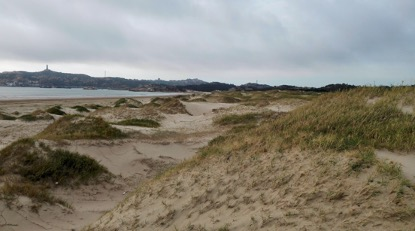
\includegraphics{../figs/sand_buried_plants.jpg}}}\hspace{5pt}
  \subfloat[\textit{C. equisetifolia} danmaged by sand burial.]{%
  \resizebox*{6cm}{!}{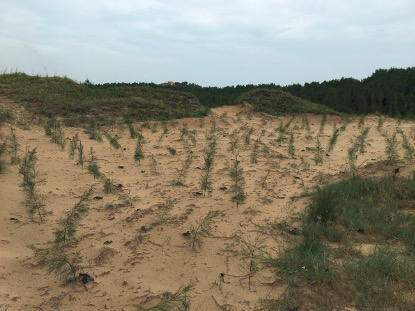
\includegraphics{../figs/damaged_trees.jpg}}}
  \caption{(a) Intensive sand burial on the \textit{Spinifex littoreus} nebkhas on Pingtan island after typhoon Soudelor (1513) landed in Putian City, Fujian Province, China in August, 2015. (b)The nebkhas formed by \textit{Spinifex littoreus} was stabilized by the planting of an invasive species Casuarinas equisetifolia seedlings on Pingtan Island, Fujian Province, China.} 
  \label{sample-pic}
\end{figure}

\label{Introduction-5}
% 我们的研究假设和研究思路
% 我们认为不同的沙埋情形将改变植株的生长方式,是该植物能够适应台风带来的强烈沙埋的关键性因素。
In this study, we assume that the different sand burial changes the growth process of \textit{S. littoreus}, which is the key factor for the plants to adapt to the intense sand burial. Then, the vertical height of ramets, horizontal length of stolons, and biomass allocation of adventitious roots, stems and leaves on stolons of \textit{S. littoreus} under different sand burial levels were simulated and measured in a field experiment, in a growing season on Pingtan Island, Fujian Province, South China.


\section{Material and Methods}
\subsection{Study area}

\begin{figure}
  \centering
  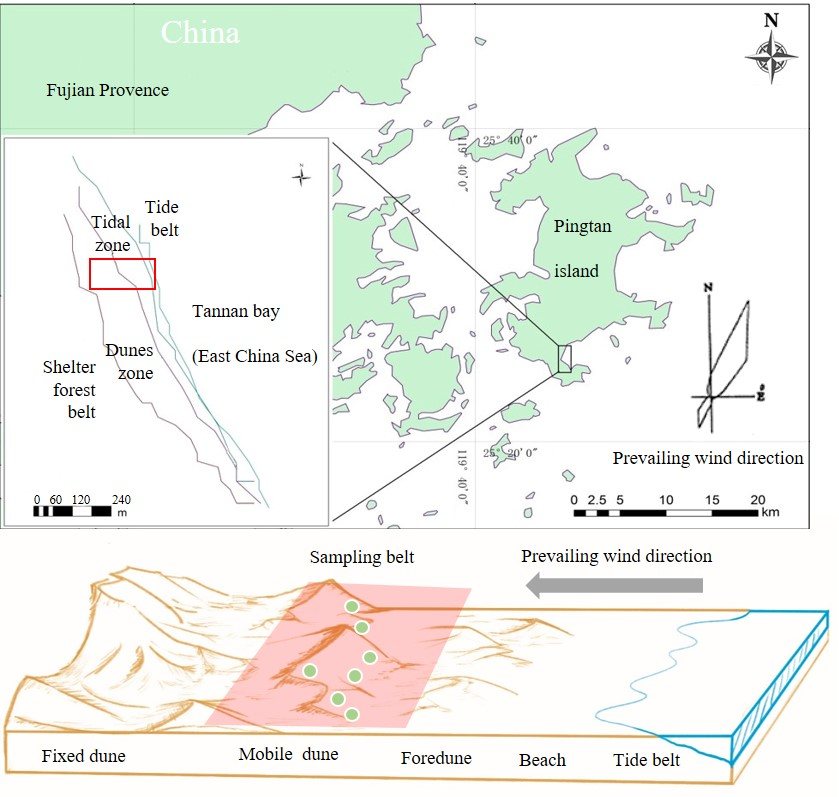
\includegraphics[scale=0.8]{../figs/study_area.jpg}
  \caption{Schematic diagram of the field experiment} 
  \label{fig:map}
\end{figure}

Pingtan island is located on the eastern coast of Fujian province, South China, with a sub-humid and oceanic monsoon climate. The study area is situated in the southeast of Pingtan island $(25^{\circ}26'36''-25^{\circ}26'48''N, 119^{\circ}46'09''-119^{\circ}46'21''E)$, and is usually regarded as hosting the most well-preserved coastal sand dunes in China (Figure~\ref{fig:map}) 
\citep{xian-jiDiurnalVariationCharacteristics2017}. 
Annual average temperature is 19.5℃, and precipitation is 1151 mm. The Monsoon is the dominant wind in this area, SE in the summer and NE in the winter, with an annual average wind speed of $6.9 m/s$. A total of 106 typhoons made landfall on Pingtan island from 1981 to 2019, average 2.65 times per year, and mainly they occur in July to September. The maximum wind speed can be up to $32.7 m/s$, ultimately leading to the severe sand burial on the psammophytes in this period. Soil is mainly composed of medium to fine sand, with well-sorted grains. Sediments are transported by the wind and intercepted by the ramets and stolons of \textit{S. littoreus}, and a discrete dune mound or hummock was usually formed by aeolian sand deposition within an isolated plant or group of plants \citep{hespCFDFlowDynamics2019}, ultimately developing into a 300 m wide nebkha dominated foredune zone (Figure~\ref{sample-pic}). \textit{S. littoreus} is the dominant species in the study area and the auxiliary plants including \textit{Oenothera drummondii}, \textit{Cynodondactylon}, \textit{Pluchea pteropoda}, and \textit{Sesuvium portulacastrum}. 



\subsection{Methods}
Field experiments were carried out in July, 2016, in Tannan bay, Pingtan Island (Figure~\ref{fig:map}). One study belt without the interruption of animals, pollutants, and apparent human activities was selected in the center of the coastal sand dunes. Considering most of the \textit{S. littoreus} were distributed on the windward slopes, 35 healthy plants with uniform size and comparable age were selected on the windward slopes were chosen for study. All the observed plants can be well distinguished from surrounding plants, and the height of vertical ramets and the length of stolons were all similar with each other before the burial treatments. Stolons of plants on the windward slopes were selected, and labeled with a red cord at points 1/3 and 2/3 of the length from the stem base to the apex of the stolons. Weeds around the selected plants were manually cleared, and wooden frames 20 cm in height (similar to the height of stolons) were set around the selected plants. Later, all the observed plants were fixed with a label, and its serial number was recorded on the label and wooden baffles respectively in order to facilitate periodic measurements later. The few adventitious roots present on the stolons of the observed plants were completely eliminated, the height of vertical ramets and length of stolons were measured separately before the experiments began. Later, all the plants were buried with sand from the nearby dunes according to a variety of different treatments (Figure~\ref{fig:diagram}). 


\begin{figure}
  \centering
  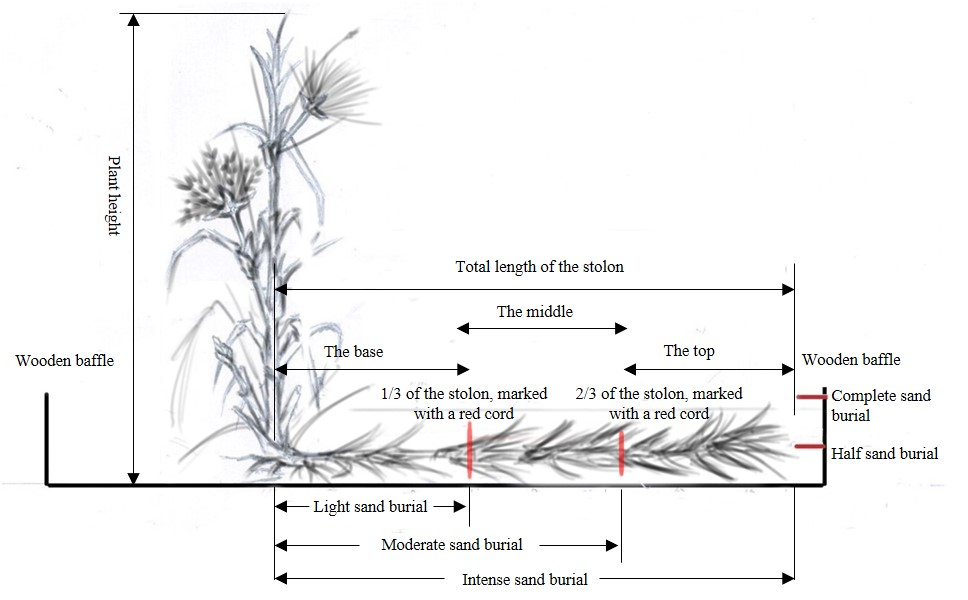
\includegraphics[scale=0.5]{../figs/diagram.jpg}
  \caption{Schematic diagram of the sand burial treatments of the samples} 
  \label{fig:diagram}
\end{figure}

\begin{table}
  \tbl{Sand burial treatments of the plants.}
  {\begin{tabular}{lrrr} 
  \toprule
   Treatment & Burial depth & Burial level \\ 
  \midrule
   CG & No sand burial & No sand burial \\
   HL & Half & Light \\
   HM & Half & Moderate \\
   HI & Half & Intense \\
   CL & Complete & Light \\
   CM & Complete & Moderate \\
   CI & Complete & Intense \\
  \bottomrule
  \end{tabular}}
  \label{tab:treatment}
\end{table}

While control groups (CG) had not been buried by sand artificially, and other groups were buried in different ways. Since the height of vertical ramets of \textit{S. littoreus} is relatively high, it is naturally impossible for them to be completely buried in the sand. The treated \textit{S. littoreus}, thus, only the stolons of which were buried at different depths and levels (see Figure~\ref{fig:diagram} and Table~\ref{tab:treatment}). Moreover, some adventitious roots on the stolons of selected plants were observed only a few days after sand burial, so the growth parameters of plants were dynamically investigated in 5, 9, 13, 17, 20 days after the sand burial to investigate the response of \textit{S. littoreus} to severe sand burial over a short time scale.

During the measurements, the sand burying the plants was carefully removed to one side in a wooden baffle, and the height of the vertical ramets, the length of the stolons and adventitious roots were all measured with a tape. After measurements (in minutes generally), all the plants were buried again with the previous sand. When the experiments were finished, both above and below ground biomass of plants were collected and separated according to the label on the stolons. Then all the samples were taken to the laboratory, and the roots, stems and leaves were separated from the stolons, dried in the oven with a temperature of 65℃ for about 24 h until the weight was constant, and then weighed with an analytical balance (accuracy: $0.0001g$).

All the data were calculated with average according to all the replications with standard error as measurement of variability. The results were analysed with Python3 and package Pingouin. For each observed variable, we used repeated measure ANOVA analysis to test if the experimental treatments were verified due to time, and checked the significance $(P<0.05)$.

\section{Results}

\subsection{Influence of sand burial on growth processes of \textit{S. littoreus}}

\begin{figure}[!h]
  \centering
  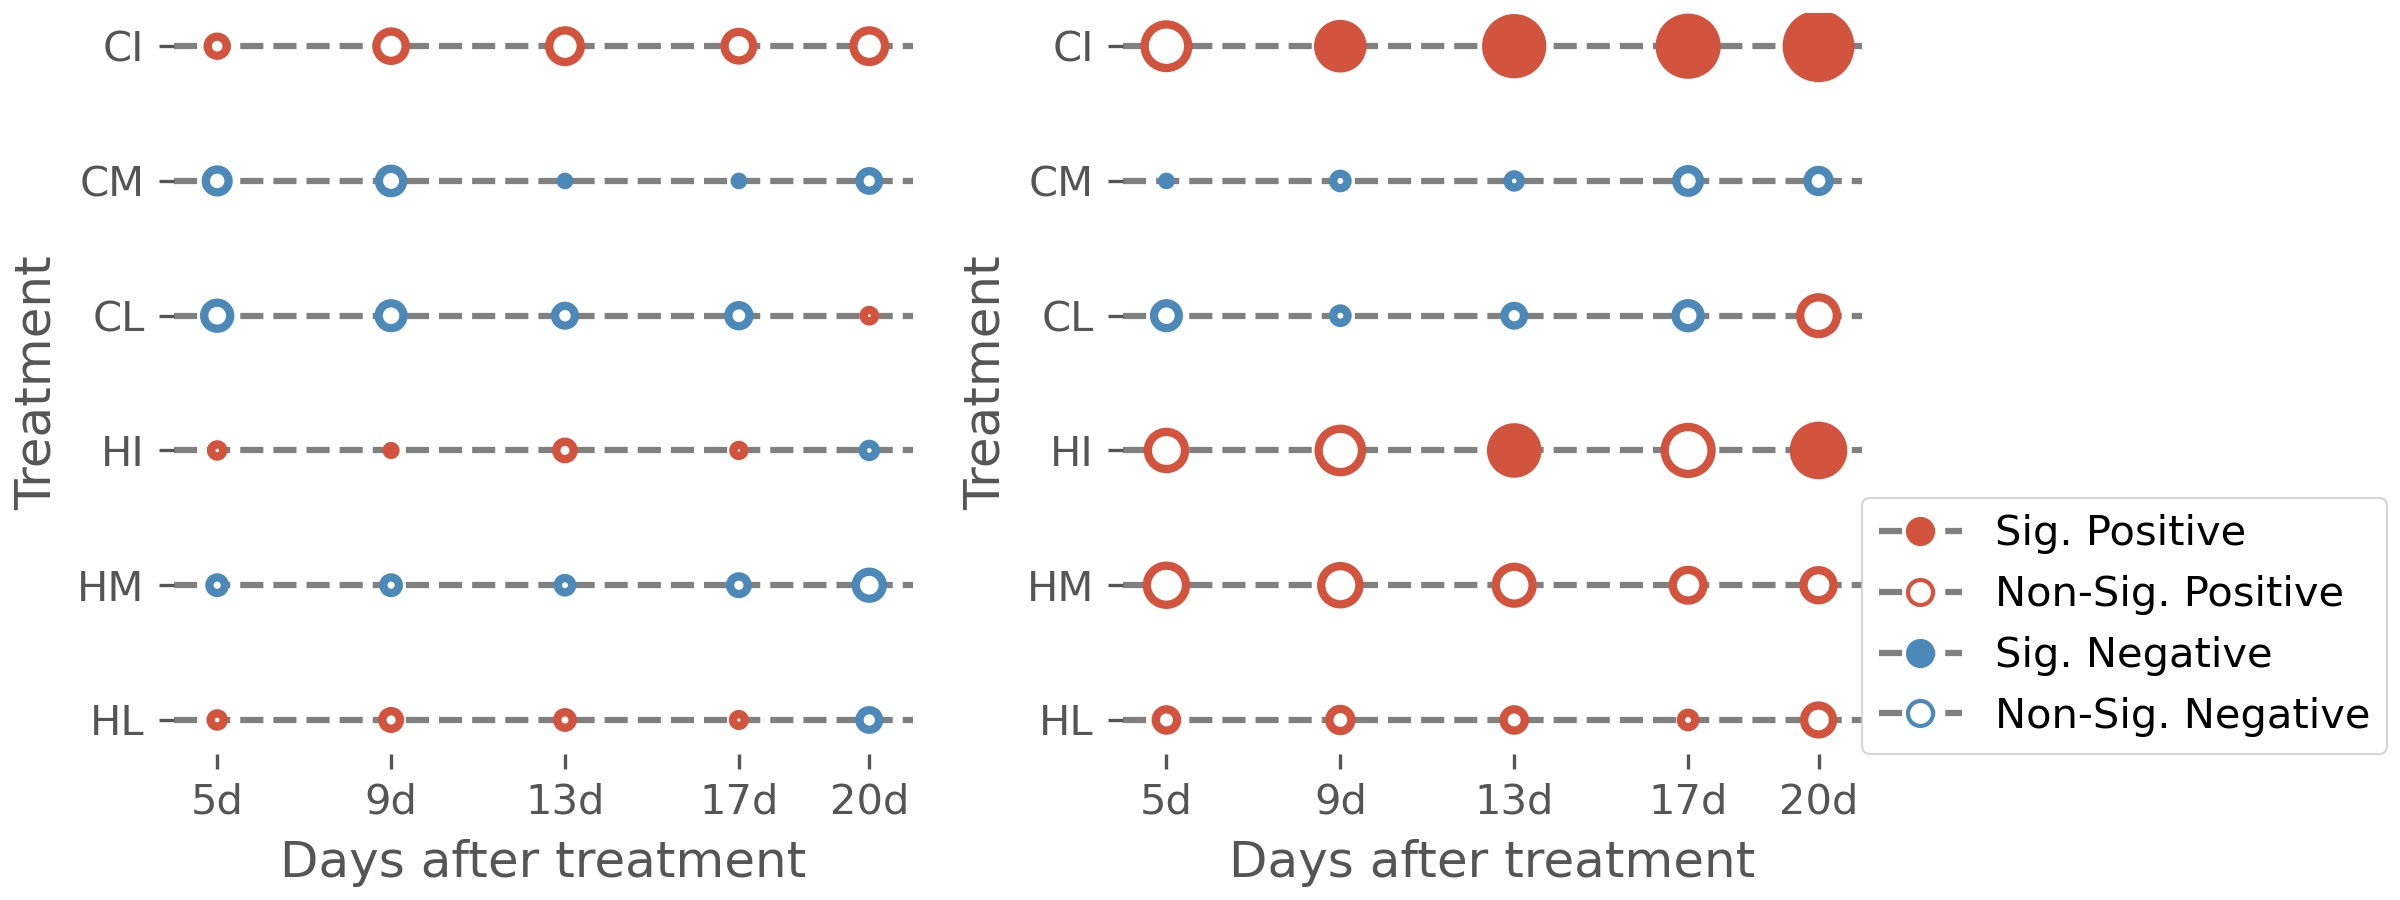
\includegraphics[scale=0.8]{../figs/grid_differences.jpg}
  \caption{
    % 不同沙埋处理下,植株的株高生长(A)与匍匐茎生长(B)同空白对照组之间的差异变化。
    Difference in ramets height growth (\textbf{A}) and horizontal stolons (\textbf{B}) between control group (CG) and different sand burial treatments. The blue dots refer negative (less than CG) while the red dots refer positive (larger than CG) differences. The fulfilled dots are significant different in statistic ($P<0.05$) and size of the dots denotes the size of difference.  
  } 
  \label{fig:lattice}
\end{figure}

\begin{figure}[!h]
  \centering
  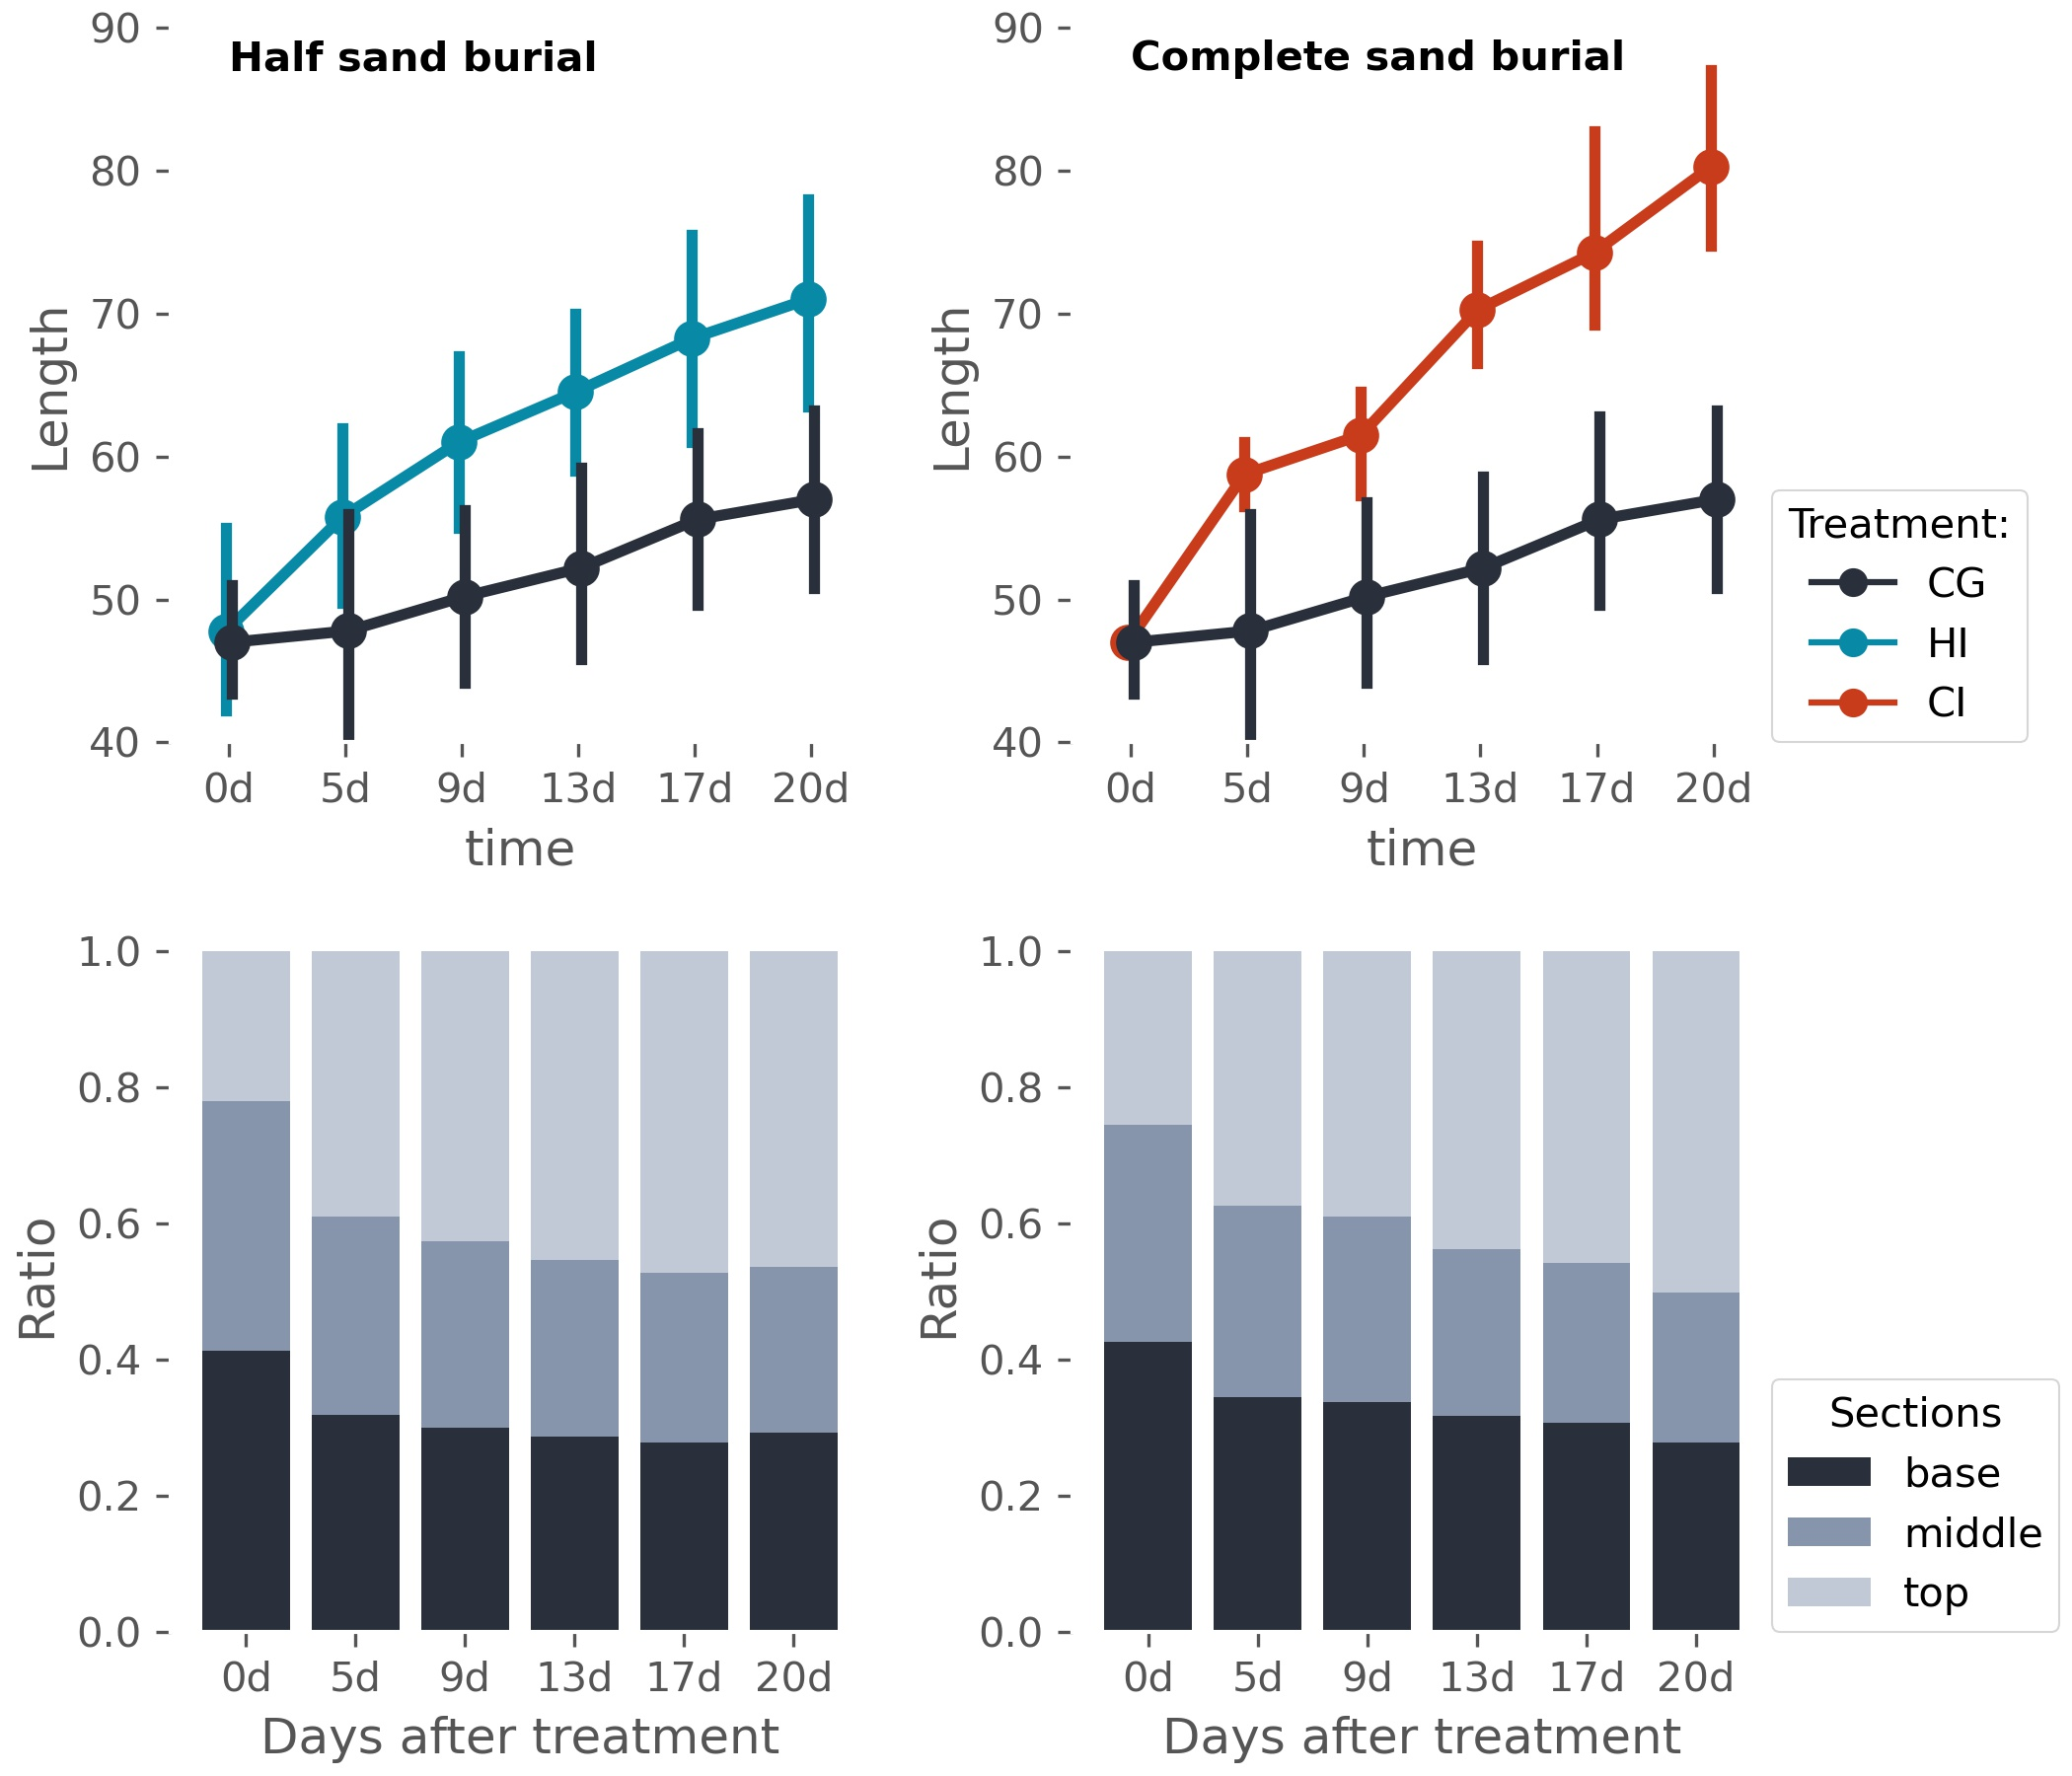
\includegraphics[scale=0.8]{../figs/growth_process.jpg}
  \caption{
    Growth process of horizontal stolons with half intense (HI) group and complete intense (CI) group plants.
    \textbf{A} growth of horizontal stolons' length of HI group, compared with the control group (CG).
    \textbf{B} growth of horizontal stolons' length of CI group, compared with the control group (CG).
    \textbf{C} growth of different sections of horizontal stolons' length of HI group.
    \textbf{D} growth of different sections of horizontal stolons' length of CI group.
  }
  \label{fig:growth}
\end{figure}

% 不同的沙埋处理下的老鼠楽株高的生长过程与空白对照之间没有显著差异(图1A),但沙埋对老鼠楽匍匐茎的伸长生长产生了显著影响(图1B)。
With different treatments, there was no significant difference between the growth of ramets height, but with significant effects on the growth of horizontal stolons when intense half sand burial (HI) and complete intense sand burial (CI) (Figure~\ref{fig:lattice}).
While the significant effect of CI occurred after 9 days after sand burial treatment, the significant effect of a HI group occurred at 13 days and 20 days after sand burial. 
% CI组不仅时间效应出现的更早,而且对水平stolons生长的促进作用也大于HI组,在20天砂埋试验结束时,其stolons长度显著增加24.56\%和40.79\%。
Not only did the time effect appear earlier with the CI group, but also had a greater promoting effect on the growth of horizontal stolons than the HI group, with significant increases in stolons' length of 40.79\% and 24.56\% respectively at the end of 20-day sand burial experiment (Figure~\ref{fig:growth} A and B).
% 其伸长生长过程都在不断增加顶端1/3长度所占的比例,而基部长度占比和中段的长度占比均匀下降(图2C-D)。
During the elongation growth process, the proportion of the length of the top 1/3 (apex) increased continuously, while the proportion of the length of the base and the length of the middle sections decreased uniformly (Figure~\ref{fig:growth} C and D).

\subsection{Influence of sand burial on the biomass allocation}
\begin{figure}
  \centering
  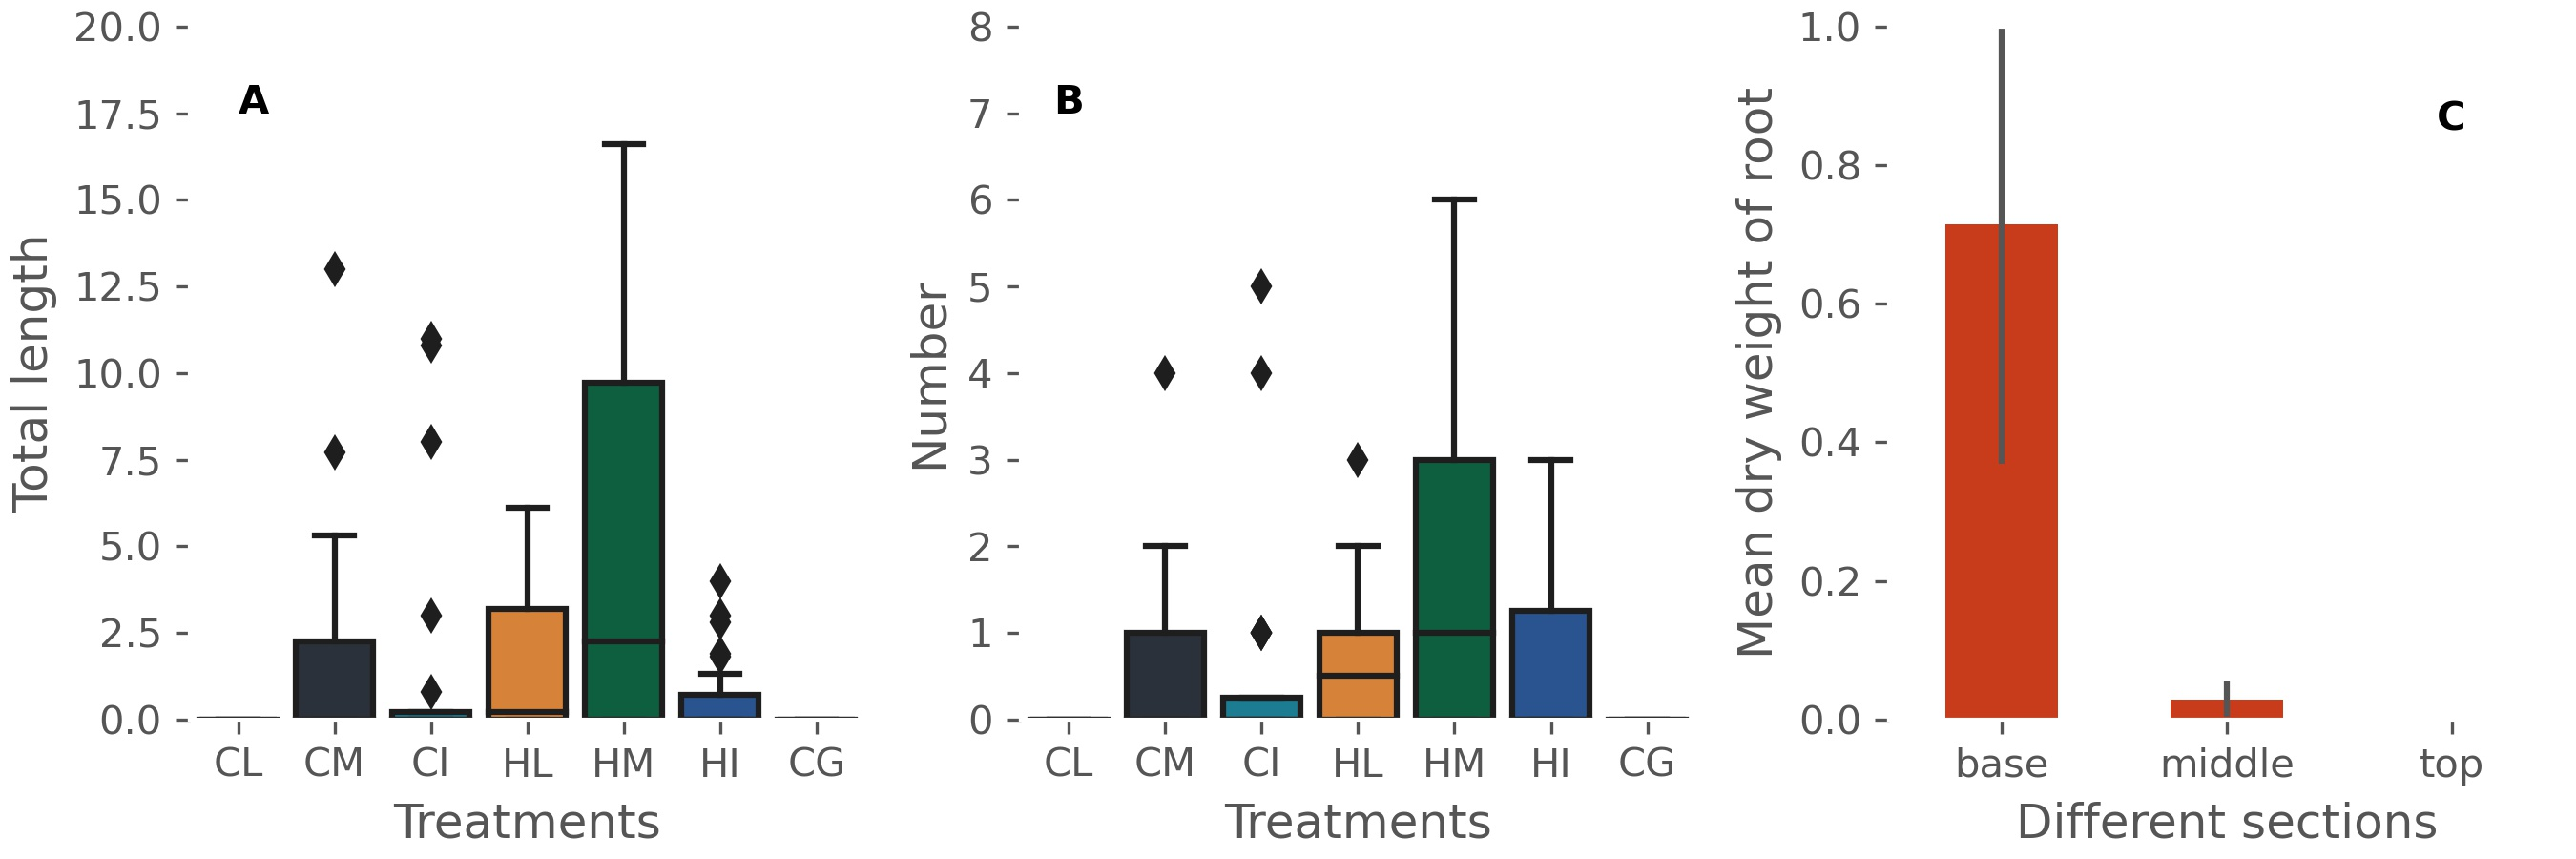
\includegraphics[scale=0.6]{../figs/roots.jpg}
  \caption{
    \textbf{A.} Total length of adventitious roots under different sand burial treatments.
    \textbf{B.} Number of adventitious roots under different sand burial treatments.
    \textbf{C.} Mean dry weights in different sections of horizontal stolons.
  }
  \label{fig:roots}
\end{figure}

\begin{figure}
  \centering
  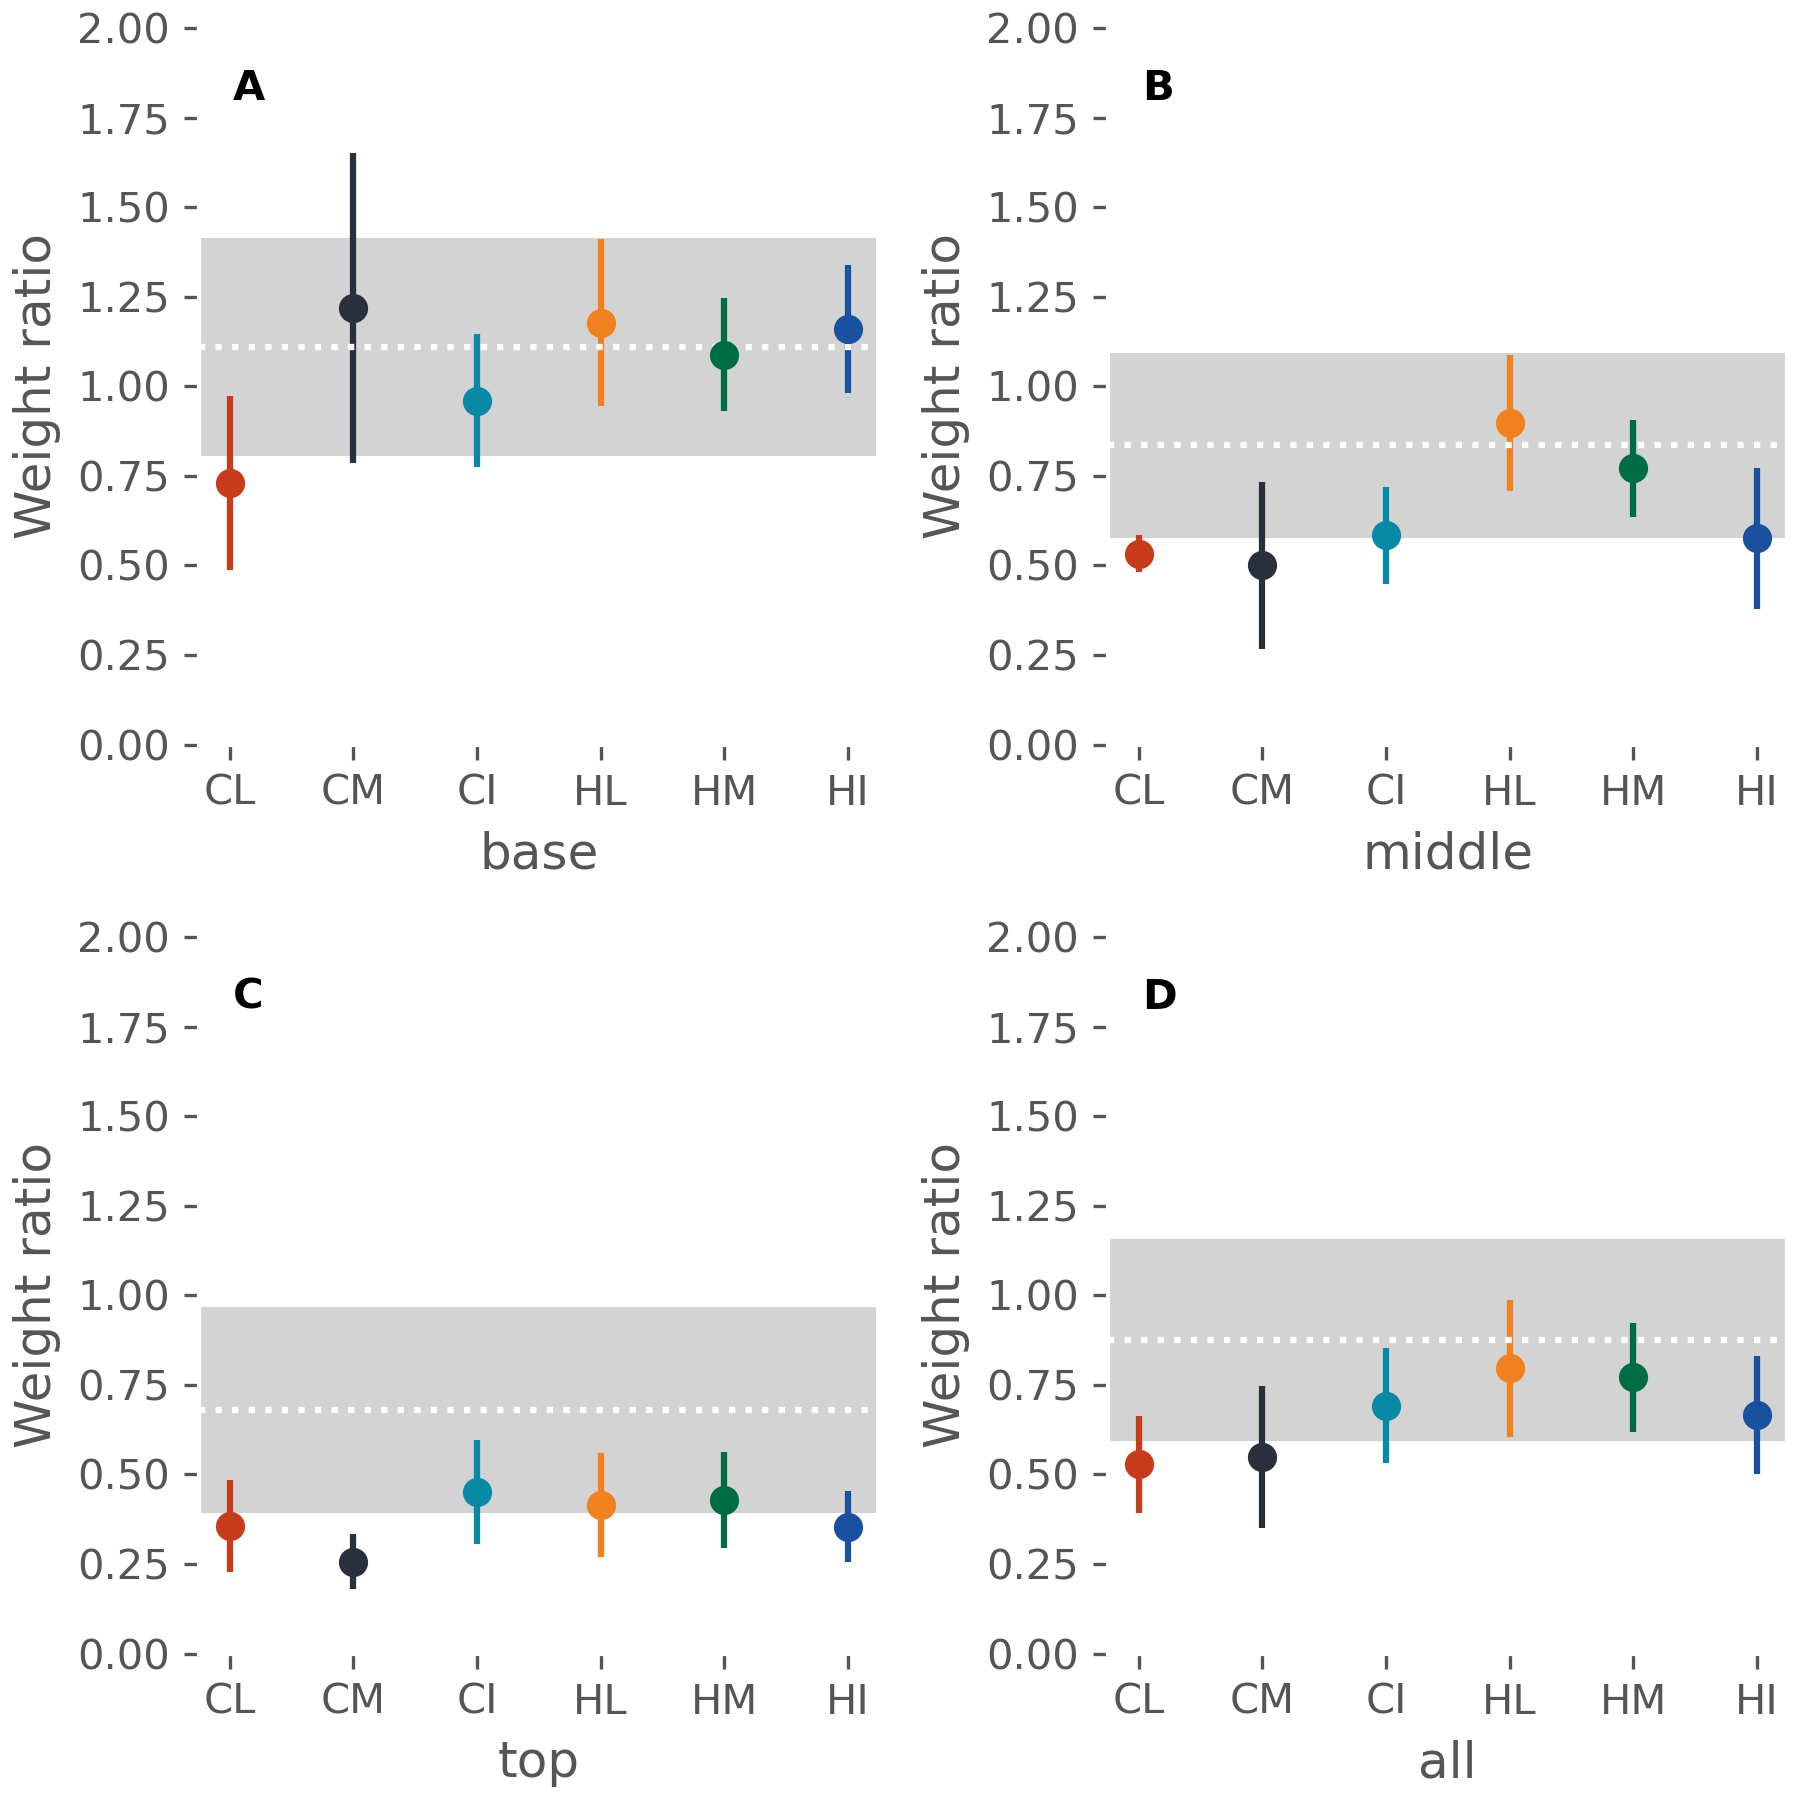
\includegraphics[scale=0.8]{../figs/ratio.jpg}
  \caption{
    Ratio between stem weights and leaf weights after the experiments under different treatments. The white lines denote mean ratio of the control group (CG) while the grey spans denote the standard error of. Weights ratio from different sections were compared one by one (\textbf{A:} base sections, \textbf{B:} middle sections, \textbf{C:} apex sections, \textbf{D:} all sections).
  }
  \label{fig:ratio}
\end{figure}

% 大多数的人工沙埋不同程度上促进了不定根的生成,无论是不定根数量还是总长度(Fig3)。
Most of sand-burial treatments promote the generation of adventitious roots to varying degrees, both in terms of the number of roots and the total length of the roots (Figure~\ref{fig:roots} A and B).
% 而且不定根主要分布在基部,顶端无不定根生成。
What's more, the adventitious roots are mainly distributed at the base and the adventitious roots are not generated at the apex (Figure~\ref{fig:roots} C).
% 经过20天的沙埋实验,老鼠楽植株茎和叶片的干重比例在不同程度上发生了改变。
After 20 days of sand-burying experiments, the ratio of dry weight between stems and leaves of \textit{S. littoreus} plant changed to varying degrees (most of which decreased in ratio of stem weight and leaf weight) under different treatments (Figure~\ref{fig:ratio}).
% 相对于空白对照组来说,沙埋使得植株将干重更多分配在茎上而非叶片上,在植株的顶端尤其明显。
Compared with the control group (CG), sand burial caused the plant to distribute dry weight more on the stem than on the leaves, especially at the top of the plant (Figure~\ref{fig:ratio} C).

\section{Discussion}

\subsection{Mechanism of \textit{\textit{S. littoreus}'} responses to severe sand burial}

% 我们的研究表明,老鼠楽对沙埋有多种不同的响应方式
Our results suggest that \textit{S. littoreus} responds to sand burial in a variety of ways: uninfluenced ramets height, increased horizontal stolons length, and changed biomass allocation.
% 这些响应方式的产生可能基于生理生态机制,我们通过和其它海岸沙生植物之间进行对比来进行探讨。
These responses based on physiological and ecological mechanisms, which we can give a glance to by comparing with other coastal sandy plants.

Sand burial has been assumed to reduce the photosynthetic area of species, which finally inhibit the plant performance in coastal sand dunes \citep{hespEcologicalProcessesPlant1991,brownMechanismsSurvivingBurial2018}. 
Species that withstand sand burial can recover very rapidly by elongating internodes in vertical shoots to overcome this physical barrier \citep{frosiniGlobalChangeResponse2012,keijsersModelingBiogeomorphicEvolution2016,quEffectsSandBurial2017,enriquezAssessingBeachDune2019}. 
However, this is inconsistent with our study, as we clearly show that sand burial on stolons of \textit{S. littoreus} in all treatments did not significantly affect the vertical growth of its conjoint ramets on the nebkhas. This is probably due to the growth characteristics of \textit{S. littoreus} which displays both vertical and horizontal development, the height of its ramets ranges from 40 to 60 cm, and it is virtually impossible to bury the entire vertical ramets by the sand sediments relative to its conjoint stolons during a single typhoon event \citep{xian-jiDiurnalVariationCharacteristics2017}. For the plants on the windward slopes, some unburied leaves will continue to provide photosynthetic substance to sustain the growth of sand dune plants even when significant burial has taken place (Figure~\ref{sample-pic}). As a result, growths of the ramets height were hardly effected by natural sand burial levels (which we simulated artificially).

Sand burial is considered as the key factor controlling the spatial distribution of specific species, and species tolerant to sand burial usually react positively to sand burial, while they respond negatively or are uninfluenced if the sand burial rate is under some threshold \citep{hespReviewBiologicalGeomorphological1989, maunAdaptationsEnhancingSurvival1994,brownMechanismsSurvivingBurial2018}. 
Our results indicated that all sand burial treatments had a significant promotion on the growth of stolons on the windward slopes, and complete sand burial had a more obvious influence than sand deposition under half sand burial. Also consistent with our field investigation, we found that the tall remets of \textit{S. littoreus} could intercept sand sediments, and its conjoint stolons were buried at different levels on nebkhas, with more sand burial on the developmental succession period than it on the stabilized succession period. The stolon length of \textit{S. littoreus} on the former was much longer than it on the latter, which can be attributed to the more dynamic sand movement on the nebkhas in the developmental or building period (Figure~\ref{fig:growth}). Qu et al \citet{quEffectsSandBurial2017} also indicated that both seedling height and the survival rate of Artemisia halodendron was enhanced by intensive sand burial, but not stimulated by moderate burial, and shallow burial even had a negative impact on its survival and growth. Species usually stimulate their growing point according to the signal of the gravity stresses \citep{ruilinAnalysisGrowthStrategy2015}, and increase their node number and internode length to escape this physical barrier \citep{maunEffectsBurialSand1996}. The stresses signal of gravity in complete sand burial was usually stronger than in half sand burial \citep{wangAdvancesStudiesMorphological2005}. 
The current study indicated that complete sand burial on stolons of \textit{S.littoreus} on windward slopes could more rapidly promote plant growth than half sand burial, particularly the growth of the stolon apex, while the base and middle section of stolons were unaffected. Since plants often obtain their energy by respiration, once the acceleration of leaf growth still cannot meet the requirement of photosynthesis and break through the sand burial, the quantity of matter will be consumed. If the species fails to synthetize the required resources, the growth of leaves in the apex will accelerate rapidly in order to produce more photosynthetic substance to adapt to the sand burial. Our results further supported this hypothesis, we found that the growth of the stolon apex of \textit{S.littoreus} was even faster as the sand burial prolonged, and complete sand burial had more obvious effects than half sand burial. This has also verified by other studies, and, for example, in \textit{Hydrocotyle vulgaris} and \textit{Lamiastrum galeobdolon}, both clonal plants, the leaf area increased with a decrease of light intensity under sand burial \citep{dongMorphologicalResponsesLocal1995}. 

Production of adventitious roots and germination of leaves on stolons can induce the variation of its substance redistribution (Shi et al. 2004), and change the biomass and growth rhythms of plants \citep{martinezResponsesDuneMosses1999,dechAdventitiousRootProduction2006}. 
Our results indicate that more adventitious roots were allocated to the stolon base, while a larger percent of leaves were observed on the stolon apex compared with other segments of stolons after sand burial. Generally, more sand burial depth can be found on the base of stolons due to sand sediments accumulated around the conjoint ramets, deeper sand burial can improve the access of roots to water, and favor the reservation of soil water \citep{yuanEffectsSandAccretion1993}. Moreover, \textit{S.littoreus} has a fibrous root system, and adventitious roots are initially produced in the node in the form of primordium. However, only the primordium in the unstretched base node of the stolons can develop well and finally break through the cuticular layer to produce the adventitious roots \citep{hochholdingerWeedsCropsGenetic2004}. 
As clonal plants, light will influence the phenotypic plasticity, and foraging behavior will change obviously in order to obtain enough resources \citep{fuResponsesGrasslandHerbaceous2013}. 
The apex is usually the least buried segment of stolons, as the photosynthetic organ, more leaves emerging on the stolon apex will reduce the risk of further sand burial, increase the light capture for photosynthesis and carbon gain \citep{yuanEffectsSandAccretion1993,shiEffectsSandBurial2004,brownMechanismsSurvivingBurial2018}, and ensure enough supply of carbohydrates for \textit{S.littoreus} to escape the sand burial. This was confirmed by Maun \citet{maunAdaptationsEnhancingSurvival1994}, who showed that leaf growth, total leaf area, number of tillers and total dry biomass were usually stimulated by partial sand burial for most of the species seedlings he studied. Gilbert et al. \citet{gilbertGrowthResponsesCoastal2008} also demonstrated that sand burial could increase the leaf area in mobile-dune species, which fully or partially replaced the lost photosynthetic leaf area, so the shoot must elongate its stem to keep newly produced leaves above the sand surface subsequent to the sand burial. The stem tissue density of species is negatively related to the maximal stem elongation rate, which will reduce the cost of stem tissue production. Production of taller but thinner shoots was observed in the young clones of Sporobolus virginicus after increased burial severity \citep{frosiniGlobalChangeResponse2012}. This was also supported by our study which indicated that whatever the sand burial treatments, the dry biomass ratio of stem to total stolons showed a decreasing trend from the base to the apex of stolons. 

\subsection{Significance of \textit{\textit{S. littoreus}'} adaptation to sand burial}

% 凭借上述机制,我们的结果表明老鼠楽能够有效在近地表被严重的沙埋情况下加速生长并存活下来。在热带和亚热带地区的海岸,频繁的台风常常为迎风坡带来数十厘米厚的沙埋,尽管这样的沙埋足以阻止大多数植物在此生长,但老鼠楽凭借其独特的适应能力在此占据来绝对优势。
With the above mentioned mechanisms, our results indicate that \textit{S. littoreus} can accelerate and survive in the presence of severe sand burial near the surface. Along the coasts of the tropical and subtropical regions, frequent typhoons often bring with them tens of centimetres of sand to the windward slope each time. Although such sand is sufficient to prevent the development of most plants, \textit{S. littoreus} are invincible here due to their unique adaptive capacity. However, if the sand burial rate is over some threshold, the growth of sand dune species will be inhibited \citep{maunEffectsBurialSand1996, shiEffectsSandBurial2004}. Our observation showed that few \textit{S. littoreus} on the leeward slopes where the sand burial are so severe that few plants can survive (Figure~\ref{fig:leeward_swale} A). This was especially true for the former, which could be attributed to the excessive sand deposition continuously depleting the stored reserves of stolons, and the increased difficulty of plants to escape from sand burial \citep{frosiniGlobalChangeResponse2012}, finally inhibiting the growth of \textit{S. littoreus} on these slopes (Figure~\ref{sample-pic}). \textit{Ammophila arenaria} was monitored with an Unmanned Aerial Vehicle by Nolet et al. \citet{noletUAVimagingModelGrowth2018}, and their data also indicated that the optimal burial rate for this species was $0.31 m$ of sand per growing season, and the maximum tolerance for \textit{Ammophila} ranges from $0.78m$ to $0.96 m$ for cover and NDVI, respectively. What's more, in the swales with less sand and better habitats, \textit{S. littoreus} were scattered, but this was already an area where a variety of plants were symbiotic and competitive (Figure~\ref{fig:leeward_swale} B).

\begin{figure}
  \centering
  \subfloat[Leeward.]{%
  \resizebox*{6cm}{!}{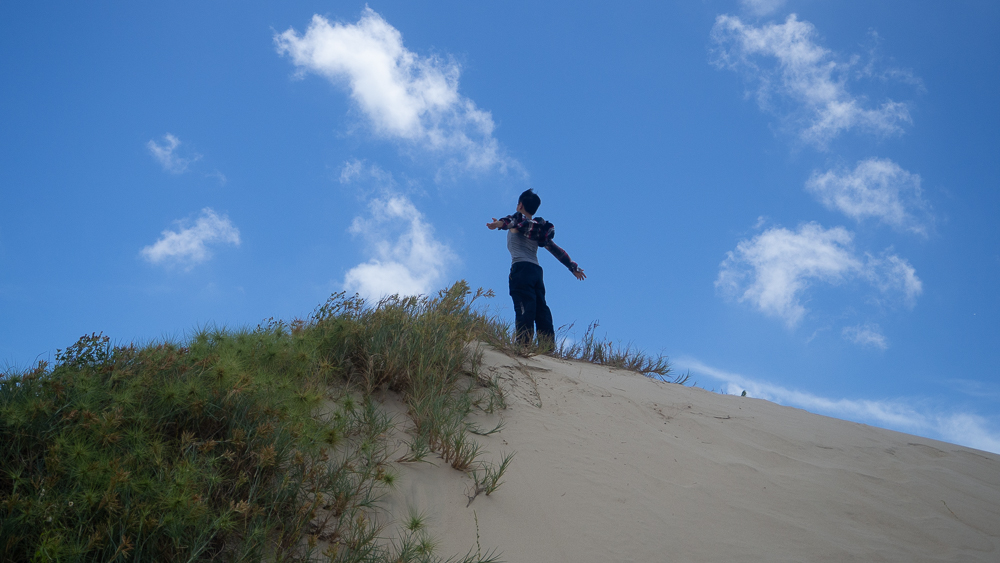
\includegraphics{../figs/leeward.jpg}}}\hspace{5pt}
  \subfloat[Swale.]{%
  \resizebox*{6cm}{!}{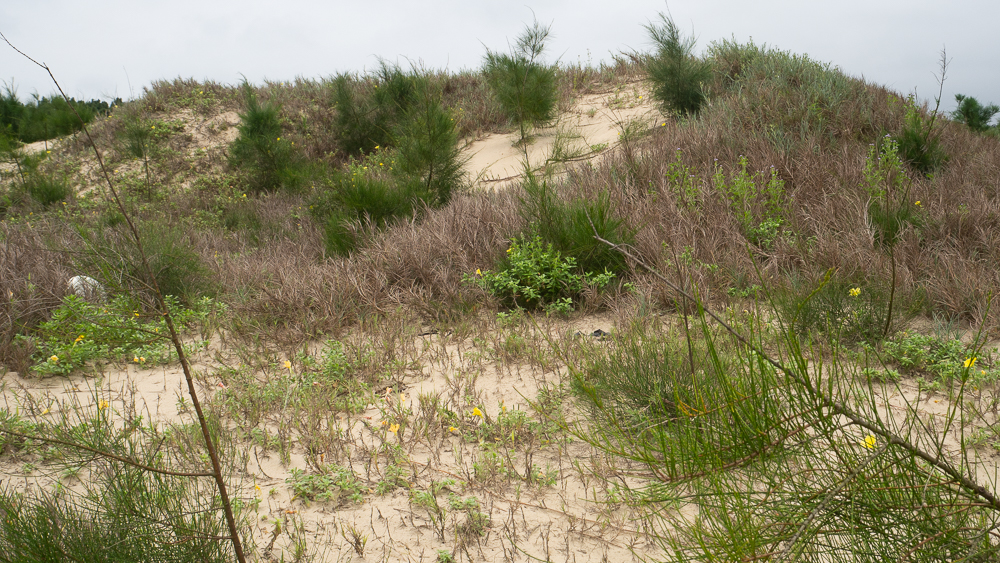
\includegraphics{../figs/swale.jpg}}}
  \caption{(a) Leeward is the most severe sand-burial position where few plants can survive there, including \textit{S. littoreus}. (b) Swales are much better habitats for plants because of little sand burial. However, \textit{S. littoreus} can not be dominant in this area because of heavy competition.} 
  \label{fig:leeward_swale}
\end{figure}

According to our study, we found that an optimal sand burial rate will not affect the survival of \textit{S. littoreus}, but enhance its growth on coastal sand dunes. This is consistent with its role as the dominant species in coastal foredunes, production of copious adventitious roots, extension of its stolons and alteration of biomass allocation pattern will all stimulate its shoot growth over the accumulating sand \citep{dechAdventitiousRootProduction2006}. 
We consider that the protective and defensive value offered by coastal sand dunes along the coastline of South China may be underestimated or neglected by the local government, and the coastal managers should allow the regular input of wind-blown sand towards this unique species for the protection and building of coastal sand dunes \citep{noletUAVimagingModelGrowth2018}, which can greatly mitigate the loss from coastal hazards in this region. So the nebkhas formed by \textit{S. littoreus} should be kept dynamic rather than stabilized by some invasive species such as \textit{C. equisetifolia} in Southeast China as such practices will lead to the loss of this native, highly adaptive species and accelerate the degradation of coastal dune systems in this region. 

\section{Conclusion}
The following conclusions may be made:

(1) All sand burial treatments had no significant impact on the growth of the height of ramets of \textit{S. littoreus}. However, the extension of its stolon was enhanced under intense sand burial (HI and CI) treatments by 24.56\% and 40.79\%, respectively.

(2) Sand burial increased the production of adventitious roots mainly in the base section of stolons, and germination of leaves on the apex of stolons, as adaptation strategies to long-last sand burials. 

(3) Based on highly adaptation to intense sand burial (even buried brought by typhoons), \textit{S. littoreus} can be one of the most protective and defensive species in the coastal ecological systems.

\section*{Acknowledgement(s)}

% An unnumbered section, e.g.\ \verb"\section*{Acknowledgements}", may be used for thanks, etc.\ if required and included \emph{in the non-anonymous version} before any Notes or References.
Thanks to Patrick Hesp for his assistance with editing our paper.

\section*{Disclosure statement}

% An unnumbered section, e.g.\ \verb"\section*{Disclosure statement}", may be used to declare any potential conflict of interest and included \emph{in the non-anonymous version} before any Notes or References, after any Acknowledgements and before any Funding information.
The authors declare no competing interests. 

\section*{Funding}

% An unnumbered section, e.g.\ \verb"\section*{Funding}", may be used for grant details, etc.\ if required and included \emph{in the non-anonymous version} before any Notes or References.
This research was supported by National Science Foundation (Grant No. 41101011; 41801101). 


% \section*{Notes on contributor(s)}

% An unnumbered section, e.g.\ \verb"\section*{Notes on contributors}", may be included \emph{in the non-anonymous version} if required. A photograph may be added if requested.


% \section*{Nomenclature/Notation}

% An unnumbered section, e.g.\ \verb"\section*{Nomenclature}" (or \verb"\section*{Notation}"), may be included if required, before any Notes or References.


% \section*{Notes}

% An unnumbered `Notes' section may be included before the References (if using the \verb"endnotes" package, use the command \verb"\theendnotes" where the notes are to appear, instead of creating a \verb"\section*").

\section{References}

\bibliographystyle{tfcse}
\bibliography{Pingtan_ecology}

\end{document}
